\documentclass[11pt]{article}

\usepackage[final]{acl}
\usepackage{times}
\usepackage{latexsym}
\usepackage[T1]{fontenc}
\usepackage[utf8]{inputenc}
\usepackage{microtype}
\usepackage{inconsolata}
\usepackage{graphicx}
\usepackage{booktabs}
\usepackage{multirow}
\usepackage{amsmath}

\hypersetup{citecolor=black, linkcolor=black, urlcolor=black}
\raggedbottom

\title{Relation or Trigger? Probing and Causally Interpreting\\a Cross-Turn Fallacy Classifier}

\author{Aaditya Sharma \\
  2019113009 \\
  IIIT Hyderabad \\
  \texttt{aaditya.sharma@research.iiit.ac.in}}

\begin{document}
\maketitle

\begin{abstract}
Motte-and-bailey and strawman are fallacies that exist only across turns: the second claim is fallacious because of how it relates to the first. Real examples are usually introduced by stock phrases such as \textit{``I never said''} or \textit{``so you're saying''}, which also open honest clarifications, so a detector can score well either by comparing the claims or by spotting the phrase. We ask which of the two a DeBERTa-v3-large encoder does. Using 683 labelled ChangeMyView exchanges and 416 minimal-pair edits that separate the relation from the phrase, we combine layer-wise probing with control tasks, minimal-pair geometry, residual-stream activation patching, attribution patching with head ablation, and LEACE concept erasure inside the forward pass. The phrase is linearly decodable from the first layer, but the fallacy signal builds up late, needs the earlier turns for motte-and-bailey, and moves 2.4 to 4 times more under relation edits than under phrase edits. Erasing the phrase direction leaves the readout unchanged, while erasing the entailment direction lowers it. Patching shows the decision forming in the reply and being written back into the first claim in layers 17 to 23, and ten late attention heads carry most of the strawman decision (AUC 0.71 to 0.44 when ablated, against 0.69 for random heads). NLI pre-training strengthens all of these causal effects. The code is available at \url{https://github.com/Ad-S/relation-or-trigger}.
\end{abstract}

\section{Introduction}

In a \textbf{motte-and-bailey}, a speaker makes a broad claim A, is challenged (C), and then retreats to a narrower, easier claim B while presenting B as the original point. In a \textbf{strawman}, a responder restates A as a distorted or stronger claim B and argues against that instead. Neither B is fallacious on its own; the fallacy lies in the relation between B and A. This makes the two fallacies harder than the single-sentence fallacy types studied in most prior work \citep{jin2022logical,habernal2018adhominem}.

These exchanges are also lexically marked. Retreats tend to begin with \textit{``I didn't say''} or \textit{``all I'm saying is''}, and strawmen with \textit{``so you're saying''}. The same phrases open fair clarifications. Our dataset was collected by searching for them, so every example contains one, fallacious or not. A classifier on such data can reach good accuracy through two different routes: comparing B with A, or reacting to the phrase. Classification scores cannot tell these routes apart. This is the setting in which shortcut learning is common \citep{gururangan2018annotation,mccoy2019right,geirhos2020shortcut}.

We look inside the model to decide between the routes. Our study is built around four research questions:
\begin{itemize}\setlength\itemsep{0pt}
\item[\textbf{RQ1}] At which layers and token positions is the fallacy label linearly decodable, once we control for what a probe can learn on its own?
\item[\textbf{RQ2}] Is that information relational (entailment, narrowing) or lexical (presence of the trigger phrase), and are the two encoded in separable directions?
\item[\textbf{RQ3}] Which layers, positions and components causally carry the decision?
\item[\textbf{RQ4}] Does an encoder pre-trained on natural language inference (NLI) reuse its entailment representations for this task?
\end{itemize}

Our contributions are: (i) 416 minimal-pair edits that either flip the label while keeping the phrase word for word, or toggle the phrase while keeping the label, with A and C fixed so that positions align for patching; (ii) a full probing, patching and erasure analysis of DeBERTa-v3-large in three variants (NLI-trained, plain and randomly initialised), using our own hook-based patching code since common interpretability libraries do not support DeBERTa; and (iii) converging evidence that the encoder routes the decision through the relation between the turns rather than through the phrase, with the causal structure localised to the reply in early and middle layers and to a small set of late heads and MLPs.

\section{Related Work}

\paragraph{Fallacy detection.} \citet{jin2022logical} classify thirteen fallacy types in single passages, and \citet{habernal2018adhominem} study ad hominem in ChangeMyView threads. Both treat fallacy detection as text classification and report accuracy. Our task is relational and cross-turn, and we focus on the mechanism rather than the score.

\paragraph{Probing.} Linear probes show what is decodable, not what is used \citep{belinkov2022probing}. We follow \citet{hewitt2019control} and report every probe against a shuffled-label control, and we compare trained encoders against a randomly initialised one and against a reply-only input.

\paragraph{Causal analysis.} Activation patching swaps hidden states between a clean and a corrupted input and measures how much of the output difference is restored \citep{vig2020causal,meng2022locating,wang2023ioi}. We follow the recommendations of \citet{zhang2024best} and use attribution patching, a first-order approximation, to rank heads and MLPs before verifying the top ones with real patching \citep{syed2024attribution,kramar2024atp}.

\paragraph{Concept erasure.} Amnesic probing removes a concept from the representation and checks whether behaviour changes \citep{elazar2021amnesic,ravfogel2020inlp}. We use LEACE \citep{belrose2023leace}, which removes all linear information about a concept with the smallest possible change to the representation, both on cached features and inside the forward pass.

\section{Data}

\paragraph{Exchanges.} We reuse the dataset from our earlier project on relational fallacy detection, built from the Winning Arguments ChangeMyView corpus \citep{tan2016winning} through ConvoKit \citep{chang2020convokit}. Candidates were mined with denial and attribution phrases, shortened to one claim per turn, and labelled by hand. Each fallacy is a separate binary task against NONE. A motte-and-bailey example has three turns (A, C, B); a strawman example has two (A, B). Table~\ref{tab:data} summarises the 683 exchanges. Besides the 188 real threads there are 20 hand-written exchanges and paraphrase and topic-transfer variants of both; every variant stays in the cross-validation fold of its source conversation.

\begin{table}[t]
\centering
\small
\begin{tabular}{lrr}
\toprule
 & Motte-and-bailey & Strawman \\
\midrule
Turns in input & A, C, B & A, B \\
Exchanges & 353 & 330 \\
\quad fallacy / NONE & 127 / 226 & 180 / 150 \\
\quad real ChangeMyView & 90 & 98 \\
Conversations (CV groups) & 97 & 101 \\
Minimal-pair originals & 104 & 104 \\
Relation edits / phrase edits & 104 / 104 & 104 / 104 \\
\bottomrule
\end{tabular}
\caption{Dataset. The minimal-pair edits are used only for analysis, never for training a readout or for a reported score.}
\label{tab:data}
\end{table}

\paragraph{Minimal pairs.} For each of 208 originals we wrote two edits of B, leaving A and C unchanged, with LLM assistance under fixed rules. A \textbf{relation edit} (cf) changes the content of B so that the label flips, while the trigger phrase is kept word for word. A \textbf{phrase edit} (ts) removes the trigger phrase, or adds one if the original had none, while the meaning and the label are kept. An example:

\begin{small}
\begin{quote}
\textbf{A:} Aptitude in math/physics and in history varies independently.\\
\textbf{B (strawman):} I'm just trying to clarify, \textit{are you saying} people who are good at math/physics are NOT good at history?\\
\textbf{Relation edit (NONE):} \ldots\ \textit{are you saying} math and history ability can vary independently, so someone can be good at one and not the other?\\
\textbf{Phrase edit (strawman):} I'm just trying to clarify: people who are good at math/physics are NOT good at history?
\end{quote}
\end{small}

\noindent Every edit was checked automatically: relation edits must keep the trigger and phrase edits must toggle it, according to an extended trigger lexicon covering the variants found in the data. Because A and C are identical within a pair, every position before B lines up, which is what patching requires.

\section{Models and Methods}

\paragraph{Encoders.} We study DeBERTa-v3-large \citep{he2023debertav3} (24 layers, 16 heads, $d=1024$) in three variants that share the architecture and tokenizer: \textbf{NLI}, the checkpoint fine-tuned on MNLI, FEVER, ANLI, LingNLI and WANLI \citep{laurer2024less}; \textbf{plain}, the pre-trained model without NLI training; and \textbf{random}, the same architecture with random weights, as a floor. Inputs are \texttt{[CLS] A [SEP] C [SEP] B [SEP]} for motte-and-bailey and \texttt{[CLS] A [SEP] B [SEP]} for strawman. We also encode B alone with the NLI model to measure how much of the signal is in the reply's own wording.

\paragraph{Frozen encoder and linear readout.} We interpret the encoder directly rather than a fine-tuned copy. In our earlier project a linear probe on the frozen NLI encoder matched full fine-tuning (AUC 0.718 vs.\ 0.674 for motte-and-bailey and 0.736 vs.\ 0.770 for strawman), so the frozen encoder already holds what the task needs. The classifier we analyse causally is a logistic-regression readout on standardised, mean-pooled layer-24 states, refit in every fold. All evaluation uses stratified 5-fold cross-validation grouped by conversation, so no example is scored by a probe or readout that saw its conversation.

\paragraph{Segments.} Using the tokenizer's offset mapping, each token is assigned to [CLS], A, C or B; within B we further mark the trigger tokens and the rest of B. Hidden states are mean-pooled over each segment, and over all tokens, at the embedding output and after each of the 24 layers.

\paragraph{Exp.~1: Probing.} For every encoder, layer and segment we train $\ell_2$-regularised logistic regression probes ($C=0.1$, 3 seeds) for four targets: the fallacy label; trigger presence; entailment, defined as the NLI model's $P(\text{A} \Rightarrow \text{B})$ above its median; and, for motte-and-bailey, narrowing, defined as $P(\text{A} \Rightarrow \text{B}) - P(\text{B} \Rightarrow \text{A})$ above its median. Each probe is paired with a control trained on shuffled labels; selectivity is AUC minus control AUC. This gives about 124,000 probes.

\paragraph{Exp.~2: Minimal-pair geometry.} With fallacy probes fitted on training conversations, we project each held-out original and its edit on the probe direction and report the shift in held-out standard deviations: signed toward the new label for relation edits, absolute for phrase edits. Confidence intervals come from a bootstrap over conversations. We also measure the cosine between fallacy and trigger probe directions.

\paragraph{Exp.~3: Activation patching.} The original is the clean input and its edit the corrupted input. The metric is the readout logit, and the effect of an edit is the gap between the clean and corrupted readouts, in readout standard deviations. Since edits change the length of B, only the aligned prefix ([CLS], A, C) can be swapped position by position. Recovery for a prefix segment at layer $l$ is the share of the gap restored by inserting its clean states into the corrupted run; recovery for B is obtained from the complementary run, where the clean input receives the corrupted prefix states, leaving only clean B. Pairs with a gap below 0.5 SD are excluded. Each run patches all 25 states of one example in a single batch, which brings the total to about 41,000 patched forward passes.

\paragraph{Exp.~3b: Heads and MLPs.} Attribution patching estimates, for every head (the 64-dimensional slice entering the attention output projection) and every MLP output, how much of the context recovery it accounts for. The top components are verified with real patching. We then mean-ablate the ten highest-ranked heads on held-out real exchanges and compare against ten random heads from the same layers.

\paragraph{Exp.~4: Erasure.} We fit LEACE erasers for the trigger, entailment and label concepts on training-fold mean-pooled states. In \emph{amnesic probing} we erase the concept from cached features and retrain the label probe. In \emph{forward erasure} we apply the eraser to every token's hidden state at layer $l$ through a hook, run the rest of the encoder, and score held-out exchanges with the unedited layer-24 readout. A random direction serves as control. The trigger eraser is fitted on all rows of a task including the phrase edits, where the phrase varies independently of the label.

All forward passes over the full grid ran on a single A100; probing used cached activations (about 1.5\,GB per encoder).

\section{Results}

\begin{figure*}[t]
\centering
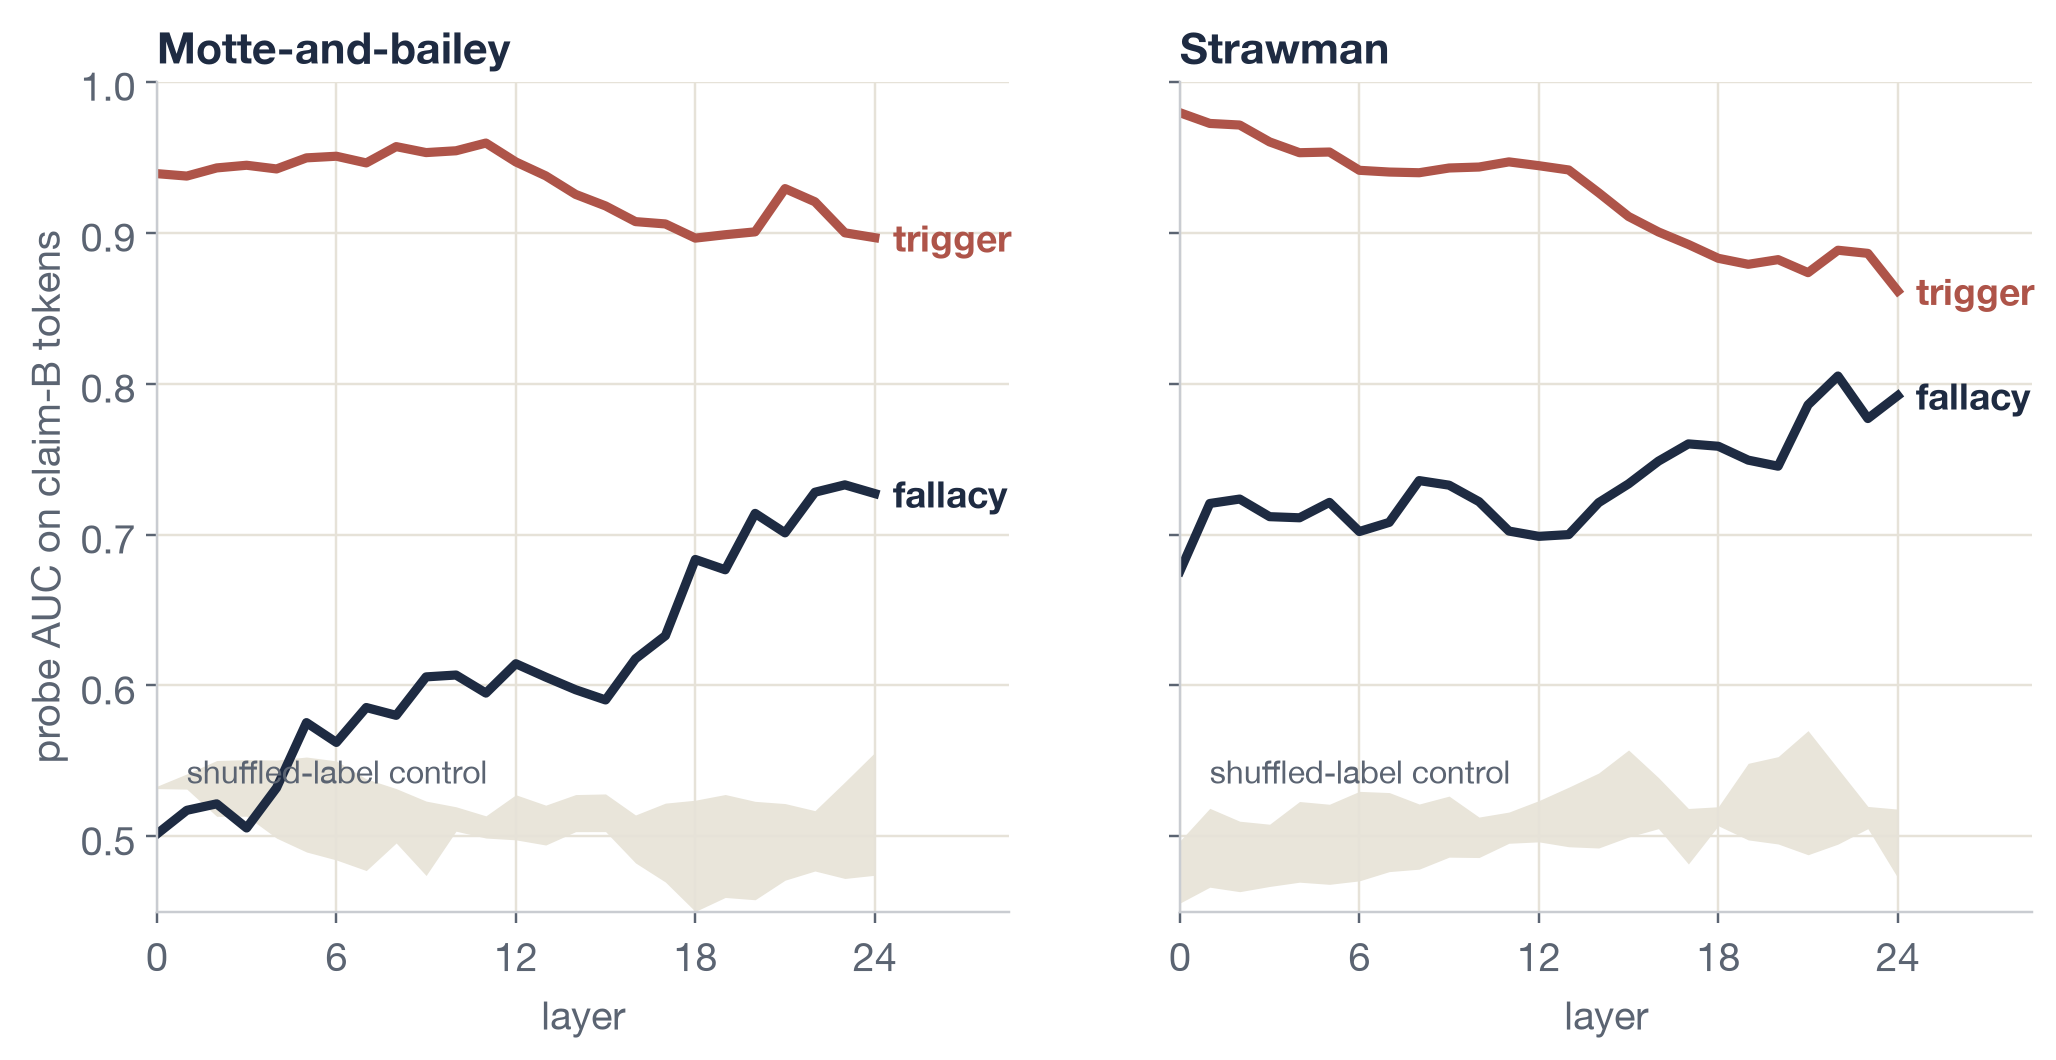
\includegraphics[width=0.92\textwidth]{figures/s_trigger_vs_label.png}
\caption{Probe AUC on B's tokens, NLI encoder. The trigger phrase is decodable from layer 0; the fallacy label rises gradually and peaks in the last third of the network. Shaded band: shuffled-label controls across all segments.}
\label{fig:probe}
\end{figure*}

\subsection{RQ1: Where the label is decodable}

Figure~\ref{fig:probe} and Table~\ref{tab:probe} give the main probing results. For \textbf{motte-and-bailey}, the label is at chance on B's tokens at layer 0 (AUC 0.50) and rises to 0.73 at layer 23, with selectivity 0.22 over the control. Encoding B alone plateaus at 0.64: the remaining signal requires A and C in the input and appears in the last third of the network (Figure~\ref{fig:context}, Appendix~\ref{app:fig}). The random encoder stays near chance. For \textbf{strawman}, B's tokens already carry signal at layer 0 (0.68), and the label reaches 0.81 at layer 22; B alone reaches 0.76. A strawman's wording, an exaggerated or absolute restatement, is partly visible in B itself, while a motte-and-bailey can only be recognised by comparison.

\begin{table}[t]
\centering
\small
\setlength{\tabcolsep}{4pt}
\begin{tabular}{llccc}
\toprule
Task & Encoder & L0 & Best (layer) & Sel. \\
\midrule
\multirow{4}{*}{M\&B} & NLI, A+C+B & 0.50 & 0.73 (23) & 0.22 \\
 & NLI, B only & 0.50 & 0.64 (17) & 0.17 \\
 & Plain & 0.50 & 0.71 (23) & 0.24 \\
 & Random & 0.50 & 0.54 (5) & $-$0.01 \\
\midrule
\multirow{4}{*}{Straw.} & NLI, A+B & 0.68 & 0.81 (22) & 0.28 \\
 & NLI, B only & 0.68 & 0.76 (20) & 0.21 \\
 & Plain & 0.68 & 0.79 (22) & 0.26 \\
 & Random & 0.66 & 0.66 (1) & 0.19 \\
\bottomrule
\end{tabular}
\caption{Fallacy-label probe AUC on B's tokens: at layer 0, at the best layer, and selectivity over the shuffled-label control at that layer.}
\label{tab:probe}
\end{table}

\subsection{RQ2: Relation or trigger}

\paragraph{The phrase is visible immediately.} Trigger presence is decodable from B's tokens at layer 0 with AUC 0.94 (motte-and-bailey) and 0.98 (strawman), and the random encoder does almost as well: this is a lexical feature that needs no processing. The fallacy direction is nearly orthogonal to it at every layer (cosine 0.04 to 0.12 for motte-and-bailey, $-$0.08 to $-$0.02 for strawman).

\paragraph{Relation edits move the representation; phrase edits barely do.} Figure~\ref{fig:geometry} shows the shift of each edit along the fallacy direction. At layer 0 the two kinds of edit are indistinguishable. From about layer 14 the curves separate. At layer 24 a strawman relation edit moves the representation by 1.30 SD toward the new label, against 0.32 SD for a phrase edit (difference 0.99, 95\% CI [0.73, 1.22]). For motte-and-bailey the relation shift peaks at 0.73 SD at layer 20, against 0.30 SD for phrase edits, with the difference significant at layer 18 (0.19, CI [0.08, 0.29]). The random encoder shows no relation shift at all.

\begin{figure*}[t]
\centering
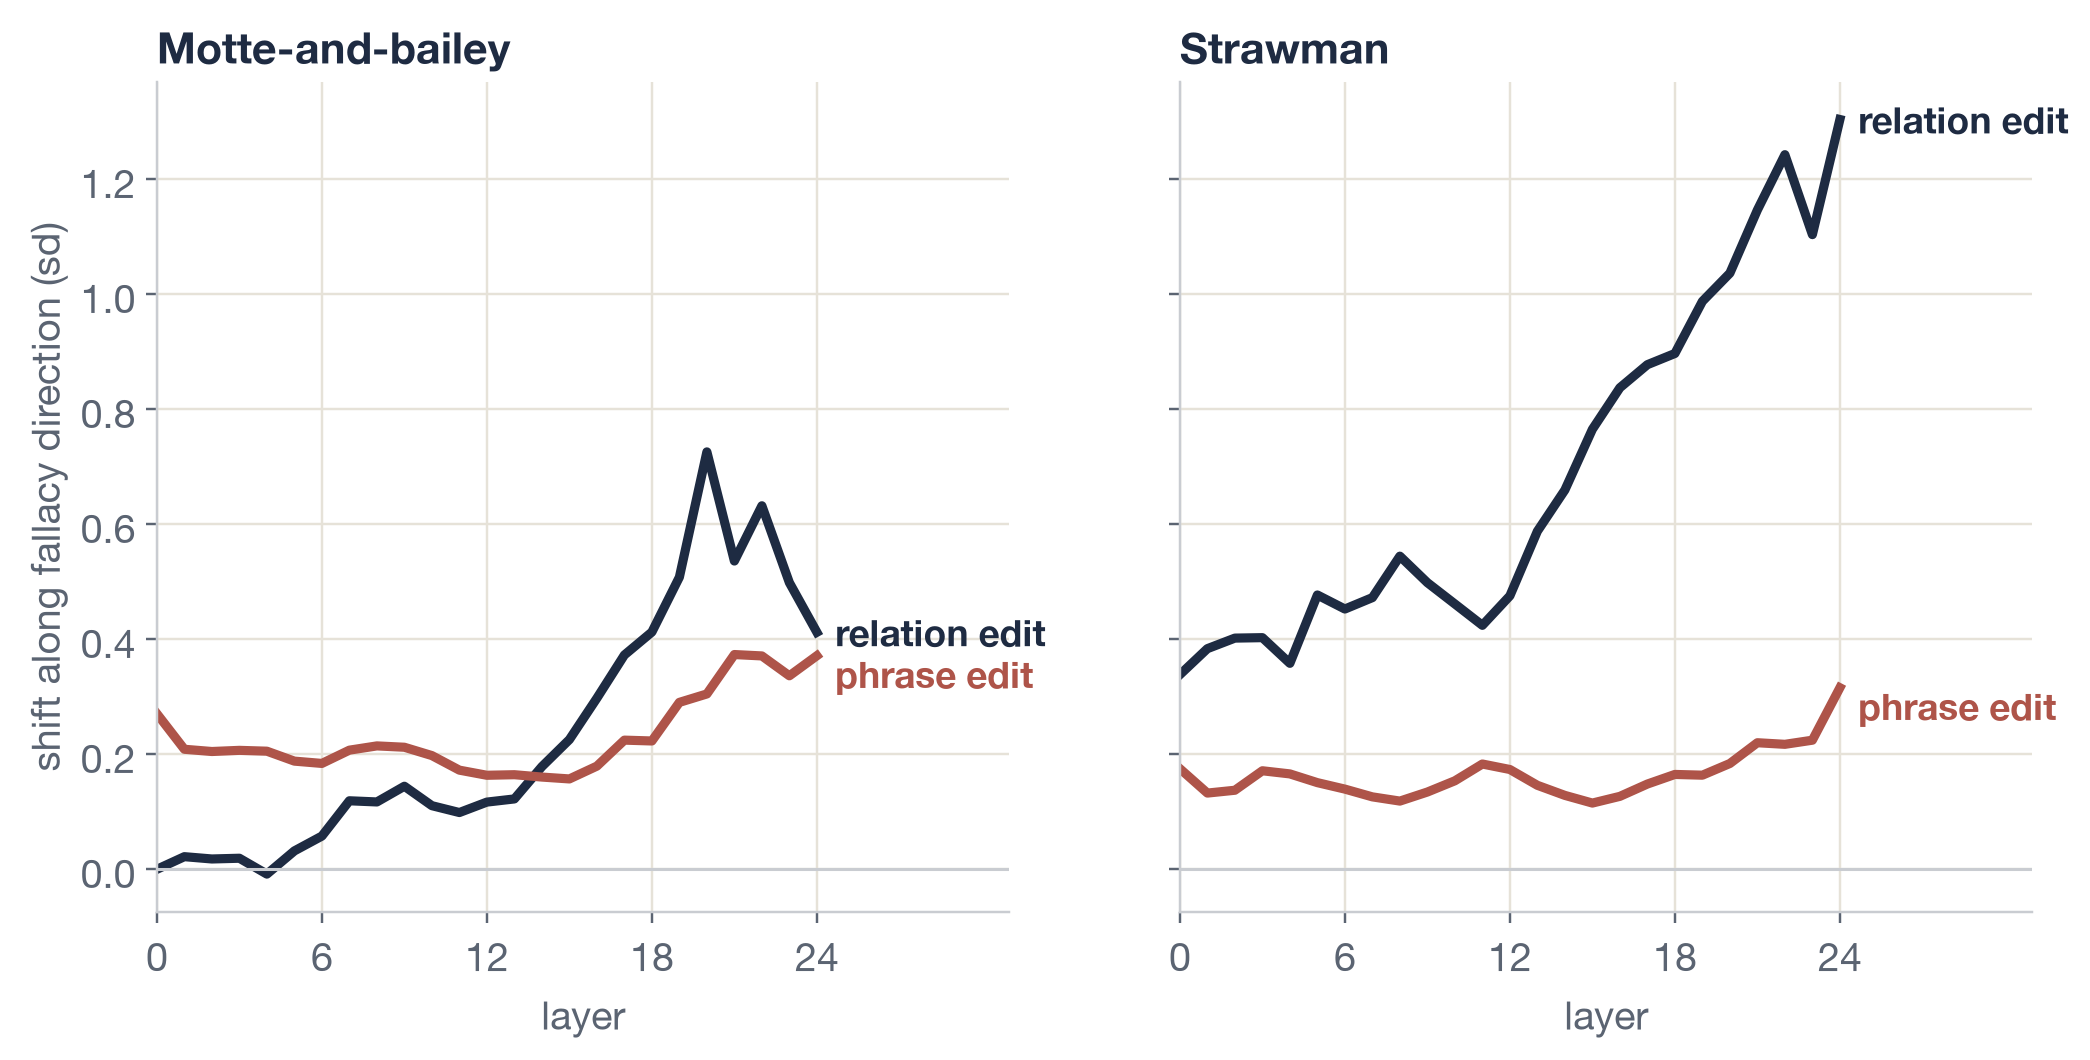
\includegraphics[width=0.92\textwidth]{figures/s_geometry.png}
\caption{Shift along the fallacy direction (held-out SD), NLI encoder, all tokens. Relation edits: signed toward the new label. Phrase edits: absolute shift.}
\label{fig:geometry}
\end{figure*}

\paragraph{Erasing the phrase changes nothing.} In amnesic probing, removing the trigger direction with LEACE changes the label probe's AUC by at most 0.01 at any layer, exactly like a random direction, while erasing the label itself drops it to 0.48 to 0.50, confirming that the eraser works. Inside the forward pass the result is the same (Figure~\ref{fig:erasure}): with the trigger erased at any layer, the downstream readout stays within 0.012 of its baseline for both tasks. Erasing the entailment direction does have an effect, concentrated in the last layers: at layer 24 strawman AUC drops from 0.713 to 0.663 and motte-and-bailey from 0.655 to 0.628, while the random direction leaves both unchanged.

\begin{figure*}[t]
\centering
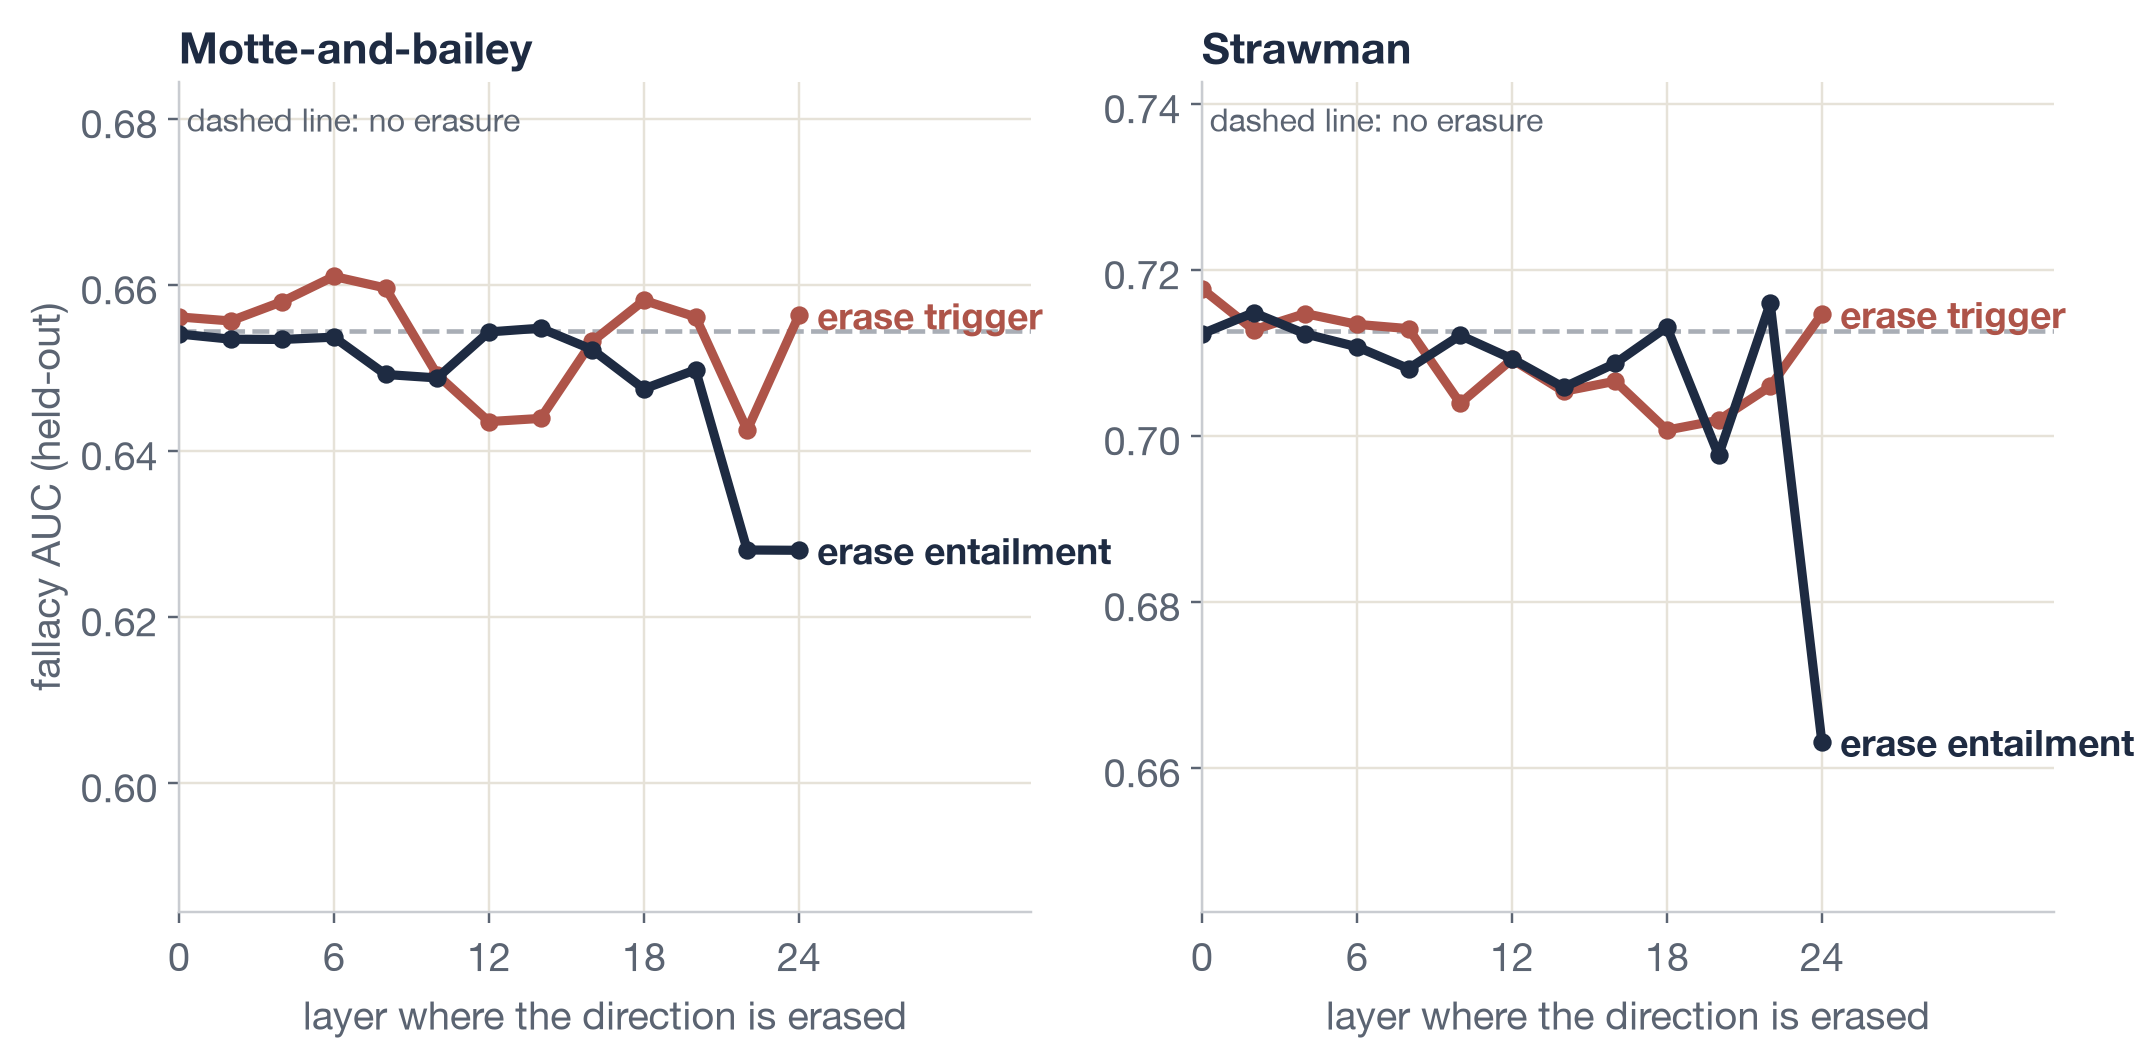
\includegraphics[width=0.92\textwidth]{figures/s_erasure.png}
\caption{Held-out readout AUC after LEACE erasure of the trigger or entailment direction at one layer, inside the forward pass (NLI encoder). Dashed: no erasure.}
\label{fig:erasure}
\end{figure*}

\subsection{RQ3: Where the decision is made}

\paragraph{Behavioural effect.} Relation edits change the readout far more than phrase edits (Table~\ref{tab:gap}). For the NLI encoder the mean gap is 1.36 SD for strawman relation edits against 0.32 SD for phrase edits, a factor of 4; for motte-and-bailey it is 1.02 against 0.35 SD, a factor of 2.9.

\begin{table}[t]
\centering
\small
\begin{tabular}{llcc}
\toprule
Encoder & Edit & M\&B & Strawman \\
\midrule
\multirow{2}{*}{NLI} & relation & 1.02 & 1.36 \\
 & phrase & 0.35 & 0.32 \\
\midrule
\multirow{2}{*}{Plain} & relation & 0.71 & 1.04 \\
 & phrase & 0.29 & 0.23 \\
\bottomrule
\end{tabular}
\caption{Mean absolute readout gap between an original and its edit, in readout SD (104 pairs per cell).}
\label{tab:gap}
\end{table}

\paragraph{Positions and layers.} Figure~\ref{fig:patching} shows where the effect lives. Up to layer 16 it sits entirely in B: B's recovery is above 0.9 for both tasks, and the prefix positions recover almost nothing. From layer 17 the information is written back into the earlier turns. By layer 23 the prefix recovers 0.46 of the gap for motte-and-bailey and 0.33 for strawman, most of it at A's tokens, with C contributing 0.12 for motte-and-bailey. [CLS] stays near zero throughout. The picture is a two-stage one: B is processed on its own positions, and its comparison with A is then written into A's positions in the last third of the network.

\begin{figure*}[t]
\centering
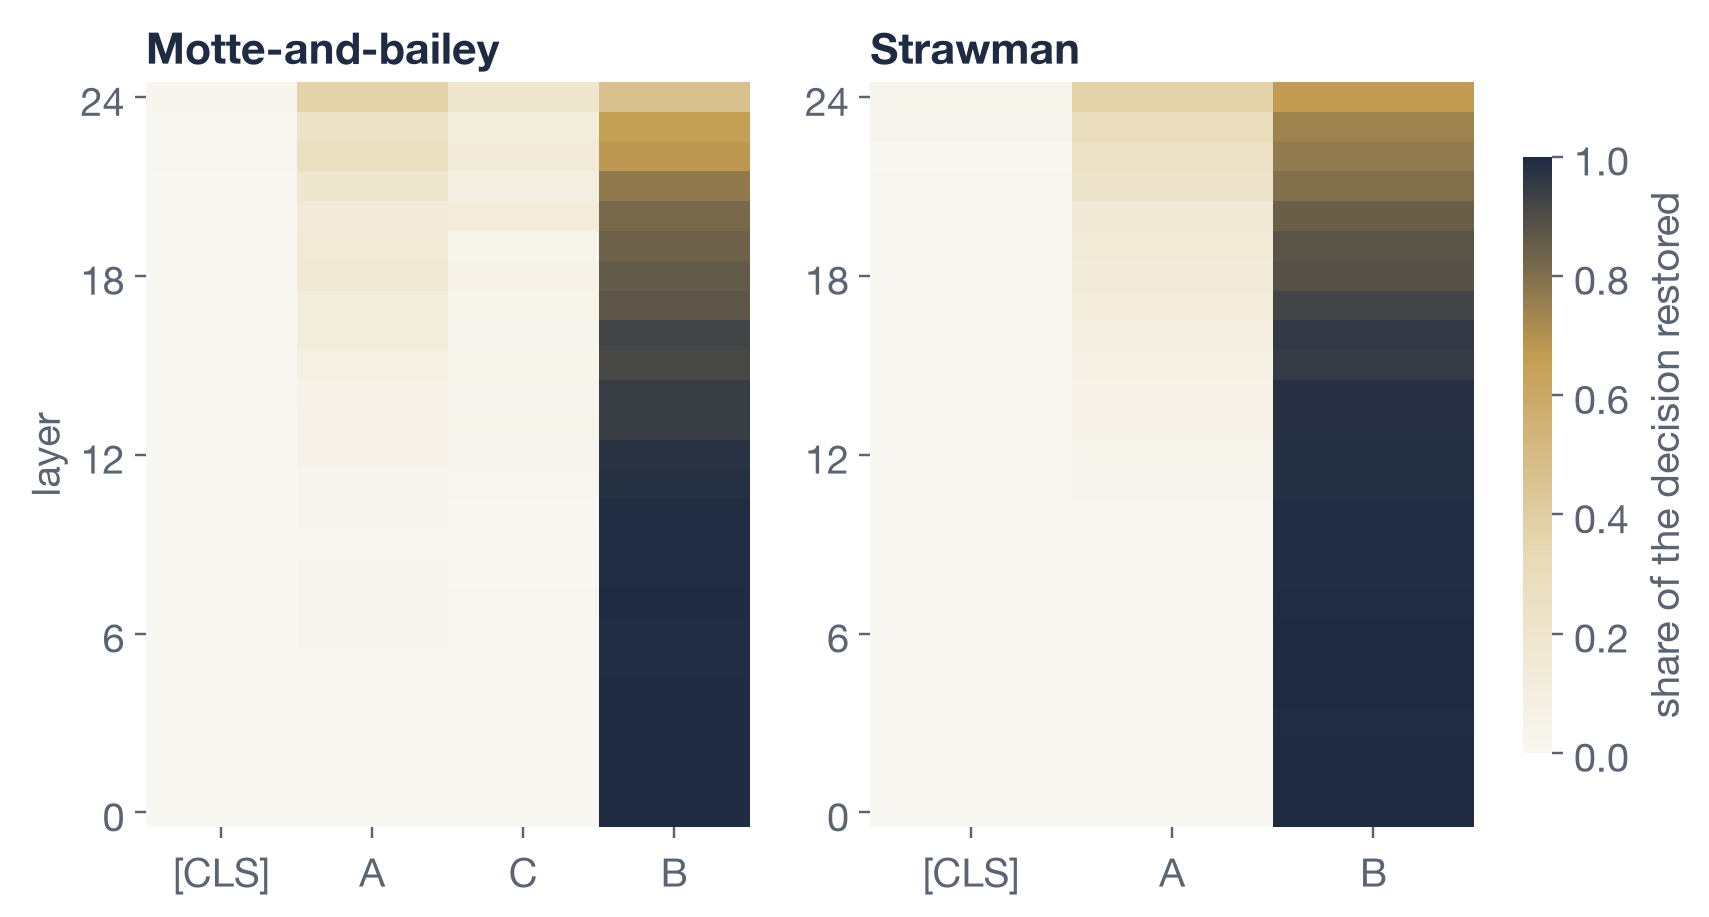
\includegraphics[width=0.78\textwidth]{figures/s_patching.png}
\caption{Median share of the relation-edit gap restored by each segment at each layer (NLI). B dominates until layer 16; from layer 17 the information appears at A.}
\label{fig:patching}
\end{figure*}

\paragraph{Components.} Attribution patching and real patching agree on the ranking (Table~\ref{tab:heads}). For strawman, the components that write B's information into the context are heads L23H11, L23H5, L20H3, L21H2 and L22H12, together with the MLPs of layers 21 to 23. For motte-and-bailey the MLPs dominate (L21 and L22, each about 0.22 recovery), followed by heads L23H8 and L23H13.

\begin{table}[t]
\centering
\small
\setlength{\tabcolsep}{4pt}
\begin{tabular}{lcc|lcc}
\toprule
\multicolumn{3}{c|}{Strawman} & \multicolumn{3}{c}{Motte-and-bailey} \\
Comp. & AtP & Patch & Comp. & AtP & Patch \\
\midrule
L23H11 & .15 & .11 & L21 MLP & .23 & .22 \\
L23 MLP & .15 & .13 & L22 MLP & .21 & .23 \\
L22 MLP & .11 & .11 & L23 MLP & .10 & .14 \\
L23H5 & .10 & .12 & L23H0 & .08 & .04 \\
L20H3 & .09 & .08 & L23H8 & .07 & .07 \\
L21H2 & .08 & .09 & L23H13 & .06 & .06 \\
\bottomrule
\end{tabular}
\caption{Top components by attribution patching (AtP) and their verified recovery with real patching (median), NLI encoder.}
\label{tab:heads}
\end{table}

\paragraph{Ablation.} Mean-ablating the ten top-ranked heads on held-out real strawman exchanges drops readout AUC from 0.713 to 0.443, below chance, whereas ten random heads from the same layers give 0.690 (Figure~\ref{fig:heads}). Ten heads out of 384 carry most of the strawman decision. For motte-and-bailey, where the MLPs dominate the ranking, head ablation does not separate from the random control (0.607 against 0.579).

\begin{figure}[t]
\centering
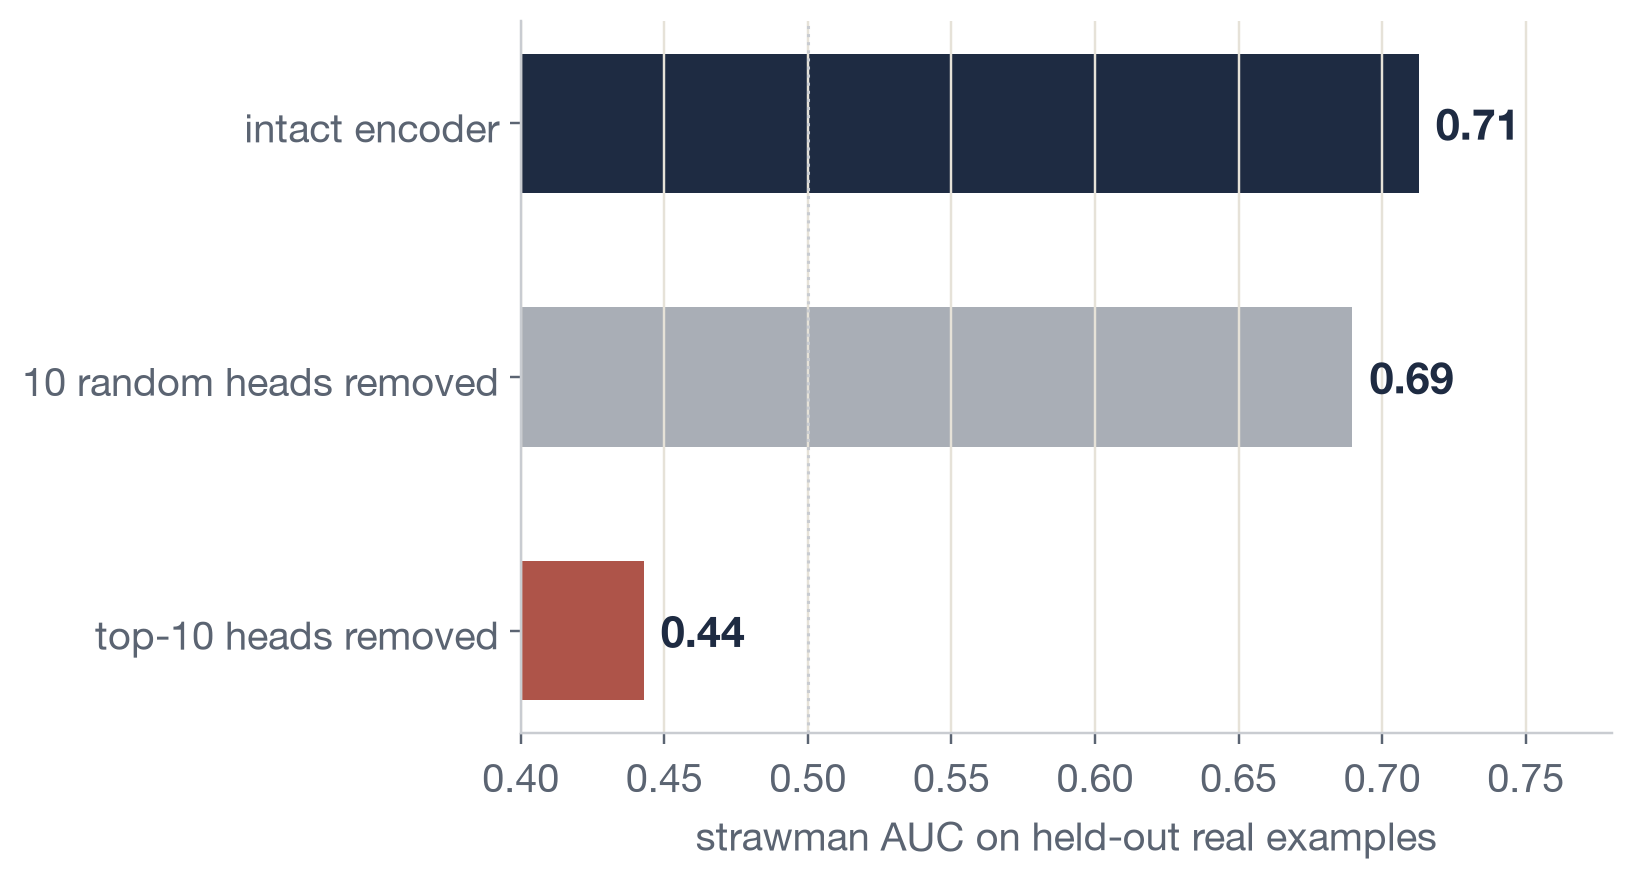
\includegraphics[width=0.9\columnwidth]{figures/s_heads.png}
\caption{Strawman readout AUC on held-out real exchanges after mean-ablating ten heads (NLI encoder).}
\label{fig:heads}
\end{figure}

\subsection{RQ4: Reuse of NLI pre-training}

The NLI encoder separates the relation from the phrase more strongly than the plain encoder on every causal measure. Its relation-edit shift at layer 24 is 1.30 against 0.92 SD for strawman, and its peak motte-and-bailey shift 0.73 against 0.50 SD. Its patching gaps are larger (Table~\ref{tab:gap}). Entailment is more decodable from it (0.90 vs.\ 0.73 on B for strawman). Its late heads are causally important, whereas ablating the top-ranked heads of the plain encoder changes AUC by at most 0.03 (0.627 to 0.603 for strawman). Erasing entailment at layer 24 costs the NLI readout 0.05 and the plain readout 0.03. Raw label decodability, by contrast, is similar for the two encoders (Table~\ref{tab:probe}): NLI training does not make the label more visible to a probe, but it makes the model's decision depend more on the relation.

At the level of single directions the overlap is small. The cosine between the fallacy direction and the entailment direction is between $-$0.20 and $-$0.03 at all layers, of the same size for the NLI, plain and random encoders, and in line with the correlation between the two labels in the data ($r=-0.12$ for motte-and-bailey, $-0.24$ for strawman). The reuse is therefore functional, through the late components that compare the turns, rather than a shared direction.

\section{Discussion}

The four experiments point the same way. The trigger phrase is the most visible feature in the encoder, decodable from the embeddings onward, yet it is orthogonal to the fallacy direction, it barely moves the readout when toggled, and removing it has no effect. The relation between the turns is what the decision depends on: relation edits shift the representation and the readout by large margins, entailment erasure lowers performance, and patching locates a specific computation in which the reply is processed first and then compared with the first claim through late attention heads and MLPs.

The two fallacies differ in a way that matches their definitions. Motte-and-bailey is invisible without the earlier turns: B alone gives much less signal, and the decision is assembled late and mostly by MLPs. Strawman is partly visible in B's wording, but the comparison with A still matters, and it runs through a small set of late attention heads whose removal destroys the decision. This is the pattern we would expect if the encoder checks whether B distorts A by attending from A's positions to B.

A practical conclusion is that the phrase-based collection of this kind of data does not, by itself, produce a phrase detector. Earlier trigger-masking experiments in our previous project suggested otherwise for a fine-tuned model; masking deletes words and breaks grammar, which is a much cruder intervention than the edits and erasure used here.

\section{Conclusion}

We asked whether a DeBERTa-v3 encoder recognises cross-turn fallacies by comparing claims or by reading a trigger phrase. Probing, minimal-pair geometry, activation patching, head ablation and concept erasure all support the relational answer. The decision forms in the reply, is written back into the first claim in layers 17 to 23, and depends on entailment information and on a small set of late heads, and NLI pre-training strengthens each of these effects.

\section*{Limitations}

The dataset has about one hundred real conversations per task, so we report effects with conversation-level bootstrap intervals and base our conclusions on large effects. The minimal-pair edits were produced with LLM assistance and validated automatically for the presence or absence of the trigger. We analyse a frozen encoder with a linear readout; the readout matches fine-tuning in accuracy, but a fine-tuned model may route information differently. The narrowing target is an NLI-based proxy, and the head-ablation control uses one random draw of heads.

\bibliography{references}

\appendix

\section{Additional Figure}
\label{app:fig}

\begin{figure}[h]
\centering
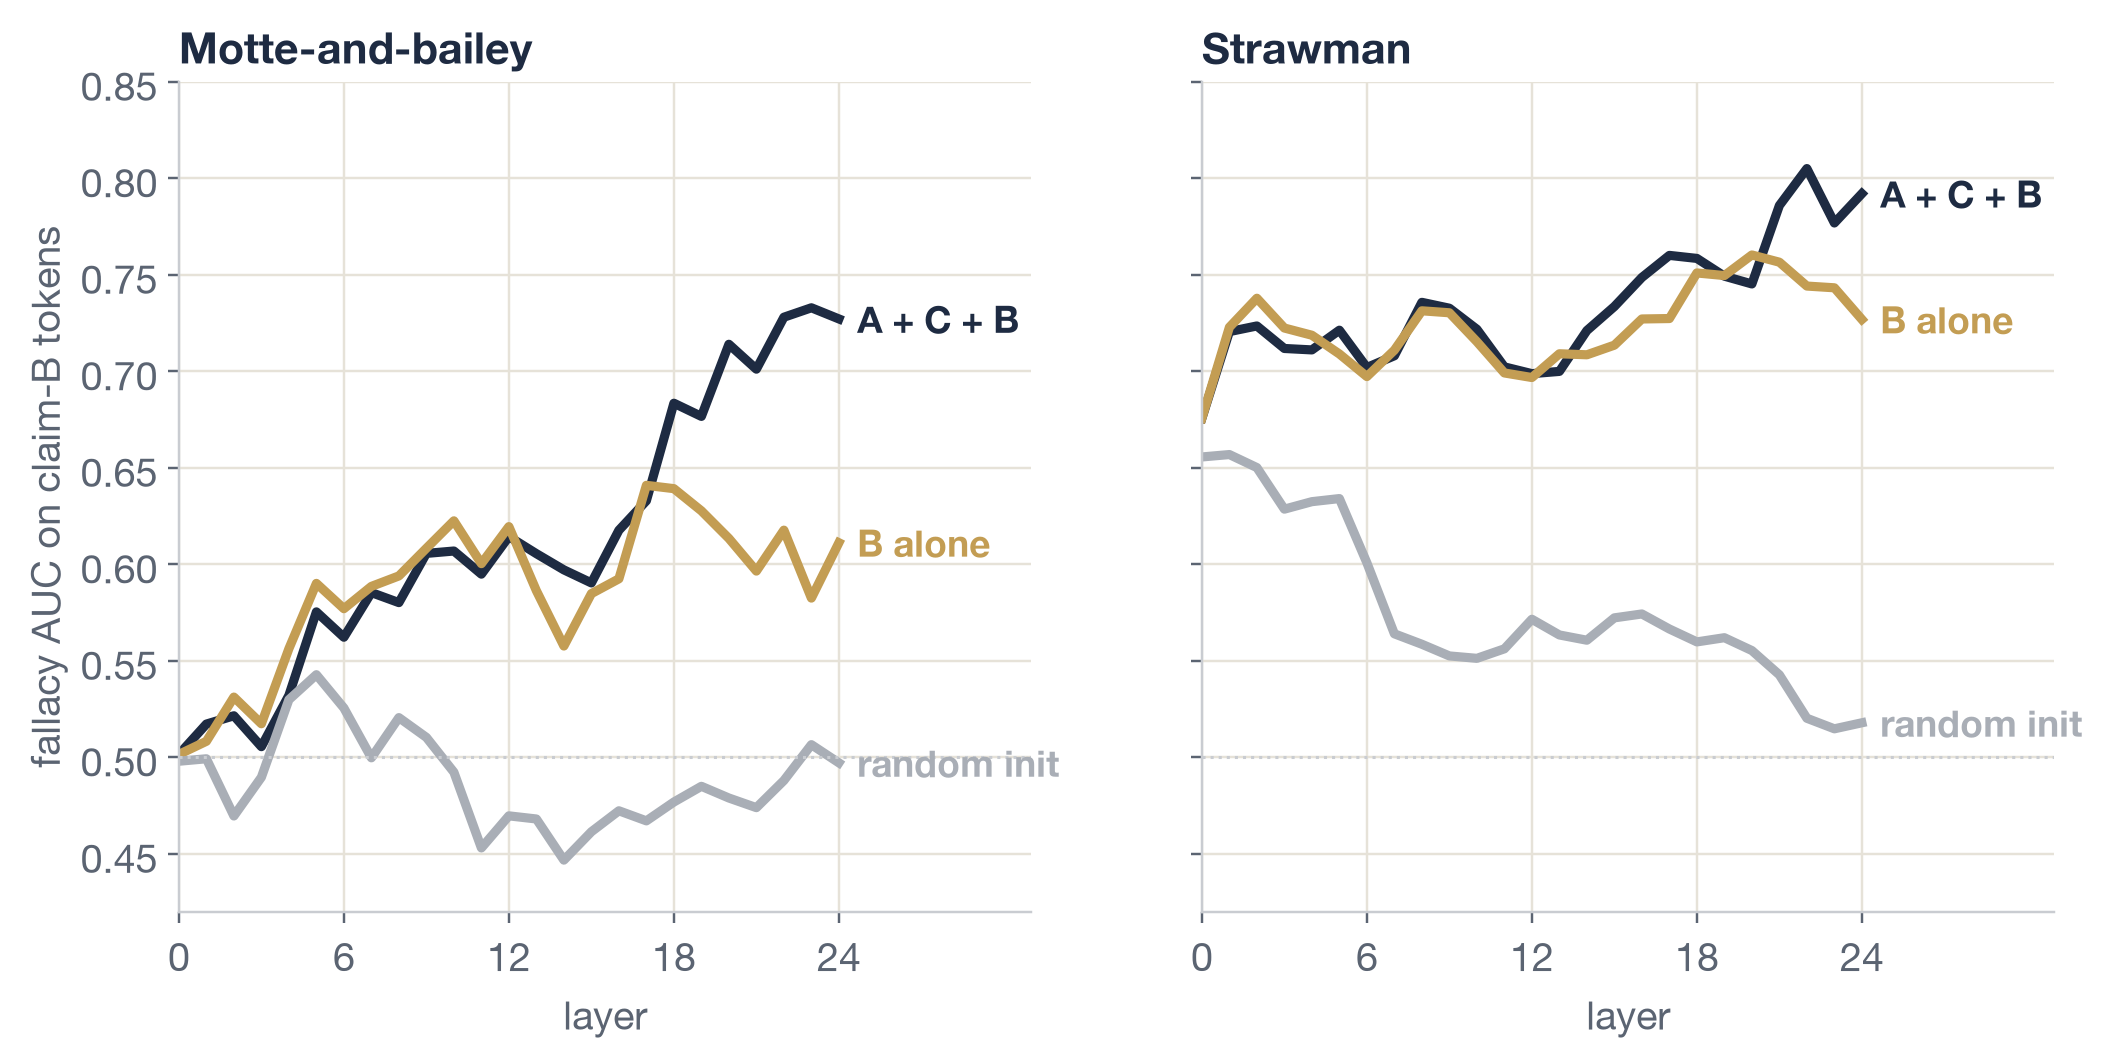
\includegraphics[width=\columnwidth]{figures/s_context.png}
\caption{Fallacy probe AUC on B's tokens for the full exchange, B alone, and the random encoder.}
\label{fig:context}
\end{figure}

\end{document}
